\documentclass[sigconf,anonymous]{aamas}

%%% == IMPORTANT ==
%%% Anonymized submission version (no author information shown).

\usepackage{balance}
\usepackage{booktabs}
\usepackage{amsfonts,amsmath,amssymb}
\usepackage{graphicx}
\usepackage{multirow}
\usepackage{xcolor}
\usepackage{pifont}

\graphicspath{{../../figures/}}

%%%%%%%%%%%%%%%%%%%%%%%%%%%%%%%%%%%%%%%%%%%%%%%%%%%%%%%%%%%%%%%%%%%%%%%%
%%% AAMAS-2027 copyright block (do not change!)

\makeatletter
\gdef\@copyrightpermission{
  \begin{minipage}{0.2\columnwidth}
   \href{https://creativecommons.org/licenses/by/4.0/}{
\includegraphics[width=0.90\textwidth]{by}}
  \end{minipage}\hfill
  \begin{minipage}{0.8\columnwidth}
   \href{https://creativecommons.org/licenses/by/4.0/}{This work is licensed under a Creative Commons Attribution International 4.0 License.}
  \end{minipage}
  \vspace{5pt}
}
\makeatother

\setcopyright{ifaamas}
\acmConference[AAMAS 2027]{Proc.\@ of the 26th International Conference
on Autonomous Agents and Multiagent Systems (AAMAS 2027)}{3--7 May 2027}{Hanoi, Vietnam}{M.~Baldoni, F.~Fang, W.~Yeoh, N.~Yorke-Smith (eds.)}
\copyrightyear{2027}
\acmYear{2027}
\acmDOI{}
\acmISBN{}

%%% OpenReview submission number (printed on first page in anonymous mode)
\acmSubmissionID{82}

\submissionType{Research Paper Track}

%%% Author-defined commands
\newcommand{\teambench}{\textsc{TeamBench}}
\newcommand{\ctrn}{\mathrm{CTR}_{\text{naive}}}
\newcommand{\ctrm}{\mathrm{CTR}_{\text{matched}}}
\newcommand{\code}[1]{\texttt{#1}}
\newcommand{\cmark}{\ding{51}}
\newcommand{\xmark}{\ding{55}}

\title[TeamBench: Assembly Protocol Determines Whether LLM Agent Teams Pay Off]{TeamBench: Assembly Protocol Determines Whether LLM Agent Teams Pay Off---A Paired, Compute-Matched Benchmark}

\begin{abstract}
Multi-agent LLM frameworks orchestrate specialized role-playing agents for complex work, yet evaluations of these systems report contradictory conclusions. We identify an overlooked confounder: \emph{how team outputs are assembled from their constituent roles is rarely controlled or even reported in paired team-vs-single evaluations.} We introduce \teambench{}, a paired individual-vs-team benchmark comprising 15 parameterized office tasks across 5 workplace scenarios $\times$ 3 coupling levels, evaluated across 7 arms: a na\"ive single agent, two compute-matched single baselines (k-round self-revision and best-of-k), and four assembly protocols (last-role output, deterministic concatenation, a dedicated integrator role, and section-slot blackboard), all applied to \emph{identical role outputs}. We run all 7 arms on \textbf{two model families} (DeepSeek-V4-Flash and Kimi-K3, 630 runs total) with Wilcoxon signed-rank tests, task-block bootstrap CIs, and BH-FDR correction. \textbf{Assembly protocol alone flips the sign of the measured team effect}, replicating across both families: geometric-mean $\ctrm$ (team quality over compute-matched single quality) spans 0.69 (last-role) $\to$ 1.55 (integrator) on Flash and 0.66 $\to$ 1.50 on K3, with the integrator arm significant on both (Flash: 1.55, 95\% CI $[1.32, 1.82]$, $p = 4.2\times10^{-7}$, $d = +0.74$; K3: 1.50, $[1.26, 1.78]$, $p = 1.2\times10^{-6}$, $d = +0.65$) and robust to call-matched comparison against best-of-k (1.56 / 1.54, both $p < 10^{-5}$). Neither k-round self-revision nor best-of-k reaches integrator-assembled quality on either model. A layer-wise decomposition shows \emph{where} the effect lives: mechanical protocols destroy the factual layer (L2 CTR 0.69--0.78, all $p<0.05$), while the integrator restores it to parity with single agents (L2 CTR $\approx$ 1.05, n.s.) and adds structural conformance (L1 saturation 96--98\% vs.\ 27--33\% for singles)---assembly determines whether the capability already present in role outputs survives into the final artifact. We also report a measurement-integrity episode: the blackboard protocol mechanically produced correct section headings without content, trivially gaming a structure-only L1 rubric in an earlier scorer version; we fix this via content-aware section scoring and publish the incident. All tasks, parameterized generators, runners, and scoring rubrics are released.
\end{abstract}

\keywords{multi-agent systems, LLM agents, benchmark, evaluation, agent orchestration, agent teams}

\begin{document}

\maketitle

\section{Introduction}
\label{sec:intro}

Frameworks for multi-agent LLM systems---AutoGen~\citep{wu2023autogen}, CrewAI~\citep{crewai2024}, LangGraph~\citep{langgraph2024}, MetaGPT~\citep{hong2024metagpt}---promise that role-specialized teams outperform a single agent on complex work. Yet the empirical evidence is deeply contradictory. Some studies report monotonic gains from more agents~\citep{li2024moreagents}; others find teams degrade quality~\citep{cemri2025masfail}; many of these papers run on non-overlapping task suites and none control for assembly. This paper argues that a large share of the contradiction is not about model capability---it is about how the final team artifact is produced from role outputs, a step rarely documented and \textbf{not previously isolated as a controlled variable over frozen role outputs in LLM team evaluation}.

We arrived at this hypothesis through our own work. In an earlier \teambench{} version (now obsolete), we adopted the engineering default of taking the last role's output as the team's artifact, and reached the headline conclusion that LLM agent teams systematically underperform individuals. But when we varied only the assembly step---leaving role prompts, task inputs, and LLM calls identical---the measured CTR swung from 0.68 to 1.52, i.e., a 0.84 point effect attributable solely to how outputs are assembled. The ``team inferiority'' finding had been a pipeline artifact, not an empirical law.

\teambench{} is a re-grounding of this question with three design principles.

\begin{enumerate}
\item \textbf{Paired-mode evaluation with assembly protocol as a first-class variable.} Every task runs in both individual mode and team mode; within team mode we explicitly compare four assembly protocols---\code{last}, \code{concat}, \code{integrator}, \code{blackboard}---over identical role outputs so assembly effects are isolated.
\item \textbf{Compute-matched single-agent baselines.} Teams consume $k$ LLM calls. We compare them not only against a 1-shot single agent but also against k-round self-revision and best-of-k selection, so any team win cannot be dismissed as ``just using more compute.''
\item \textbf{Artifact scoring with a measurement-integrity contract.} We score each delivery along three layers: L1 structural (now content-aware, \S\ref{sec:design}), L2 factual over structured answer blocks, L3 semantic via an LLM judge. The code documents every rubric change; we do not bury gaming incidents.
\end{enumerate}

\paragraph{Contributions.}
\begin{itemize}
\item \textbf{\teambench{}}, a paired individual-vs-team benchmark that isolates \emph{how} team outputs are assembled as a controlled factor over frozen role outputs: 15 tasks across 5 office scenarios $\times$ 3 coupling levels, with 150 parameterized task variants, 7 evaluation arms, and a runner with breakpoint-resume, balance-guard, and deterministic rescore tools.
\item An \textbf{artifact scoring protocol} with a documented measurement-integrity correction; $\ge$80\% of scoring weight is deterministic; closed-form definitions of Capability Transfer Rate (CTR), Coordination Overhead (CO), and Team Memory \& Structure (TMS), consistent across paper, code, and metrics docs.
\item An empirical study on \textbf{two model families} (DS v4 Flash and Kimi K3, 15 tasks $\times$ 3 seeds $\times$ 7 arms each, 630 runs total, L2 assertions active) showing that \textbf{assembly protocol flips the sign of the measured team effect on both}: geometric-mean $\ctrm$ spans 0.69--1.55 (Flash) and 0.66--1.50 (K3) over identical role outputs; the integrator arm beats both compute-matched baselines on both (vs.\ refine-k: Flash 1.55, 95\% CI $[1.32,1.82]$, $p=4.2\times10^{-7}$, $d=+0.74$; K3 1.50, $[1.26,1.78]$, $p=1.2\times10^{-6}$, $d=+0.65$; vs.\ best-of-k at identical call counts: 1.56 / 1.54), while naive engineering defaults (last-role) produce artifactual ``team-inferiority'' effects on both ($\ctrm$ 0.69 / 0.66). A layer-wise decomposition localizes the effect: mechanical protocols degrade the factual layer (L2 CTR 0.69--0.78), the integrator restores it to parity (L2 CTR $\approx$1.05, n.s.) while adding structural conformance (L1 saturation 96--98\% vs.\ 27--33\%).
\item A cross-model negative result on structured assembly: deterministic section-slot (blackboard) and raw concatenation perform near or below the single baseline on both families---on K3, mechanical protocols collapse to $Q=0$ on one aggregation task (\code{t-DATA-L-01}) across all seeds while the integrator turns the \emph{same role outputs} into a perfect artifact---because LLMs write role-specific rather than schema-matching headings; only the semantic integrator normalizes these free-form outputs.
\item Full release of tasks, parameterized generators, runner infrastructure, and scoring rubrics.
\end{itemize}

\section{Related Work}
\label{sec:related}

\subsection{Single-agent benchmarks and office-scenario evaluation}
AgentBench~\citep{liu2023agentbench}, GAIA~\citep{mialon2023gaia}, SWE-bench~\citep{jimenez2024swebench}, and OSWorld~\citep{xie2024osworld} evaluate a \emph{single} agent per task on success-oriented rubrics. TheAgentCompany~\citep{xu2024theagentcompany} is closest to us in task flavor (office work) but does not report the marginal value of adding agents.

\subsection{Multi-agent systems and their evaluation}
Orchestration frameworks~\citep{wu2023autogen,hong2024metagpt,crewai2024,langgraph2024,qian2024chatdev} report demo success rather than controlled paired comparisons. Recent scaling studies: ``More Agents\ldots''~\citep{li2024moreagents} and ``More LLM Calls\ldots''~\citep{chen2024morellmcalls} study \emph{performance scaling with agent count / LLM-call count} on single-success metrics, without separating specialization gains from compute gains. MultiAgentBench~\citep{zhu2025multiagentbench} scores collaboration behaviors, not quality transfer. Agents' Room~\citep{huot2025agentsroom} provides a structural existence proof. \citet{cemri2025masfail} contribute a MAST taxonomy of failures, including assembly-stage bugs; our work complements this by quantifying, in a controlled task space, how \emph{a single class} (output assembly) alone flips the sign of the measured team--single difference over identical role outputs.

\paragraph{Closest prior work: TeamBench of \citet{kim2026teambench}.}
Concurrent with our work, \citet{kim2026teambench} introduce a same-named but complementary benchmark (931 seeded instances, SWE-style tasks) that enforces \emph{OS-level role separation} across Planner/Executor/Verifier containers and asks whether coordination genuinely occurs; their Teamwork Necessity Index measures when teams beat solos under that separation. Our \teambench{} asks a different question on a different task distribution: given whatever role outputs a team produces, \emph{how the final artifact is assembled from them} is an unmeasured pipeline step. We freeze role outputs and vary only assembly (4 protocols) against compute-matched single baselines, yielding CTR as a paired quality-transfer measure. The two benchmarks are complementary: they test whether coordination happens; we test whether assembled artifacts preserve the capability that coordination produced.

\subsection{Team science, coordination cost, and aggregation}
Coordination theory~\citep{malone1994interdisciplinary} and Brooks' law~\citep{brooks1995mythical} explain why adding human workers can reduce throughput; \teambench{} transplants this question to LLM teams whose members share weights and pass messages losslessly~\citep{woolley2010evidence}. Debate, self-consistency, and majority voting evaluate answer aggregation of \emph{independent answers to the same question}. Assembly protocols aggregate \emph{non-overlapping role slices of a complex document} into a single artifact---a qualitatively different problem of semantic alignment, structure, and completeness.

\subsection{LLM-as-judge}
We follow MT-Bench-style judging~\citep{zheng2023judging} with a cross-vendor judge matrix and an on/off ablation (\S\ref{sec:scorer-validity}), consistent with recommended practices~\citep{guo2024survey}.

\begin{table}[t]
\centering
\caption{\teambench{} vs.\ prior agent benchmarks and multi-agent studies.}
\label{tab:comparison}
\small
\setlength{\tabcolsep}{2.5pt}
\begin{tabular}{lcccccc}
\toprule
Benchmark & Paired & Assembly & Compute- & Team & Coupling & Contam.\\
 & sing./team & contr. & matched & metrics & axis & defense \\
\midrule
AgentBench~\citep{liu2023agentbench} & \xmark & \xmark & \xmark & \xmark & \xmark & \xmark \\
GAIA~\citep{mialon2023gaia} & \xmark & \xmark & \xmark & \xmark & \xmark & \xmark \\
SWE-bench~\citep{jimenez2024swebench} & \xmark & \xmark & \xmark & \xmark & \xmark & \xmark \\
OSWorld~\citep{xie2024osworld} & \xmark & \xmark & \xmark & \xmark & \xmark & \xmark \\
TheAgentCo.~\citep{xu2024theagentcompany} & \xmark & \xmark & \xmark & \xmark & \xmark & \xmark \\
More Agents~\citep{li2024moreagents} & \xmark & \xmark & partial & single & \xmark & \xmark \\
More LLM Calls~\citep{chen2024morellmcalls} & \xmark & \xmark & \cmark & single & \xmark & \xmark \\
MultiAgentBench~\citep{zhu2025multiagentbench} & \xmark & \xmark & \xmark & behavior & \xmark & \xmark \\
Agents' Room~\citep{huot2025agentsroom} & \xmark & \xmark & \xmark & per-task & \xmark & \xmark \\
TeamBench-Kim~\citep{kim2026teambench} & \cmark & \xmark & \xmark & TNI & \xmark & \cmark \\
\textbf{\teambench{} (ours)} & \cmark & \cmark\,(4) & \cmark\,(2) & CTR/CO/TMS & \cmark\,(L/M/H) & \cmark\,(param.) \\
\bottomrule
\end{tabular}
\end{table}

\section{Problem Formulation and Metrics}
\label{sec:formulation}

Given a task $\tau \in \mathcal{T}$ with deterministic-plus-judge scoring $Q(\cdot) \in [0,1]$ and token consumption $C(\cdot)$, define on \emph{paired runs} $(a_s, a_{T,p})$ where $a_s$ is the single-agent artifact and $a_{T,p}$ is the team artifact produced under assembly protocol $p$:

\paragraph{Capability Transfer Rate (CTR).} Two variants for two baselines:
\begin{equation}
\ctrn = \frac{Q(a_{T,p})}{Q(a_s)}, \qquad
\ctrm = \frac{Q(a_{T,p})}{Q(a_{s^{(k)}})}
\end{equation}
where $a_{s^{(k)}}$ is the \emph{compute-matched} single artifact (k-round refine or best-of-k, same total LLM-call budget as team). We report CTR as the \textbf{geometric mean over paired runs} (ratio scale---arithmetic mean is biased) and 95\% bootstrap CI via 2000 block-bootstrap replications per task.

\paragraph{Coordination Overhead (CO)} $= C(a_{T,p}) / C(a_s)$; Token Ratio (TR) is synonymous. Integrator assembly overhead \emph{includes} the dedicated final LLM call.

\paragraph{Team Memory \& Structure (TMS)} $= [\![\text{L1}=1.0]\!] \wedge [\![\text{all L2 assertions pass}]\!]$. A single boolean, no partial credit.

Weights in $Q$: $Q = w_1 \cdot \mathrm{L1} + w_2 \cdot \mathrm{L2} + w_3 \cdot \mathrm{L3}$ with $w_1{=}0.50, w_2{=}0.30, w_3{=}0.20$. When the L3 judge is disabled, we renormalize to $(w_1\,\mathrm{L1} + w_2\,\mathrm{L2})/(w_1{+}w_2)$ rather than injecting a constant---this removes an additive bias that shrinks CTR toward 1 for all arms.

\section{Benchmark Design}
\label{sec:design}

\begin{figure*}[t]
\centering
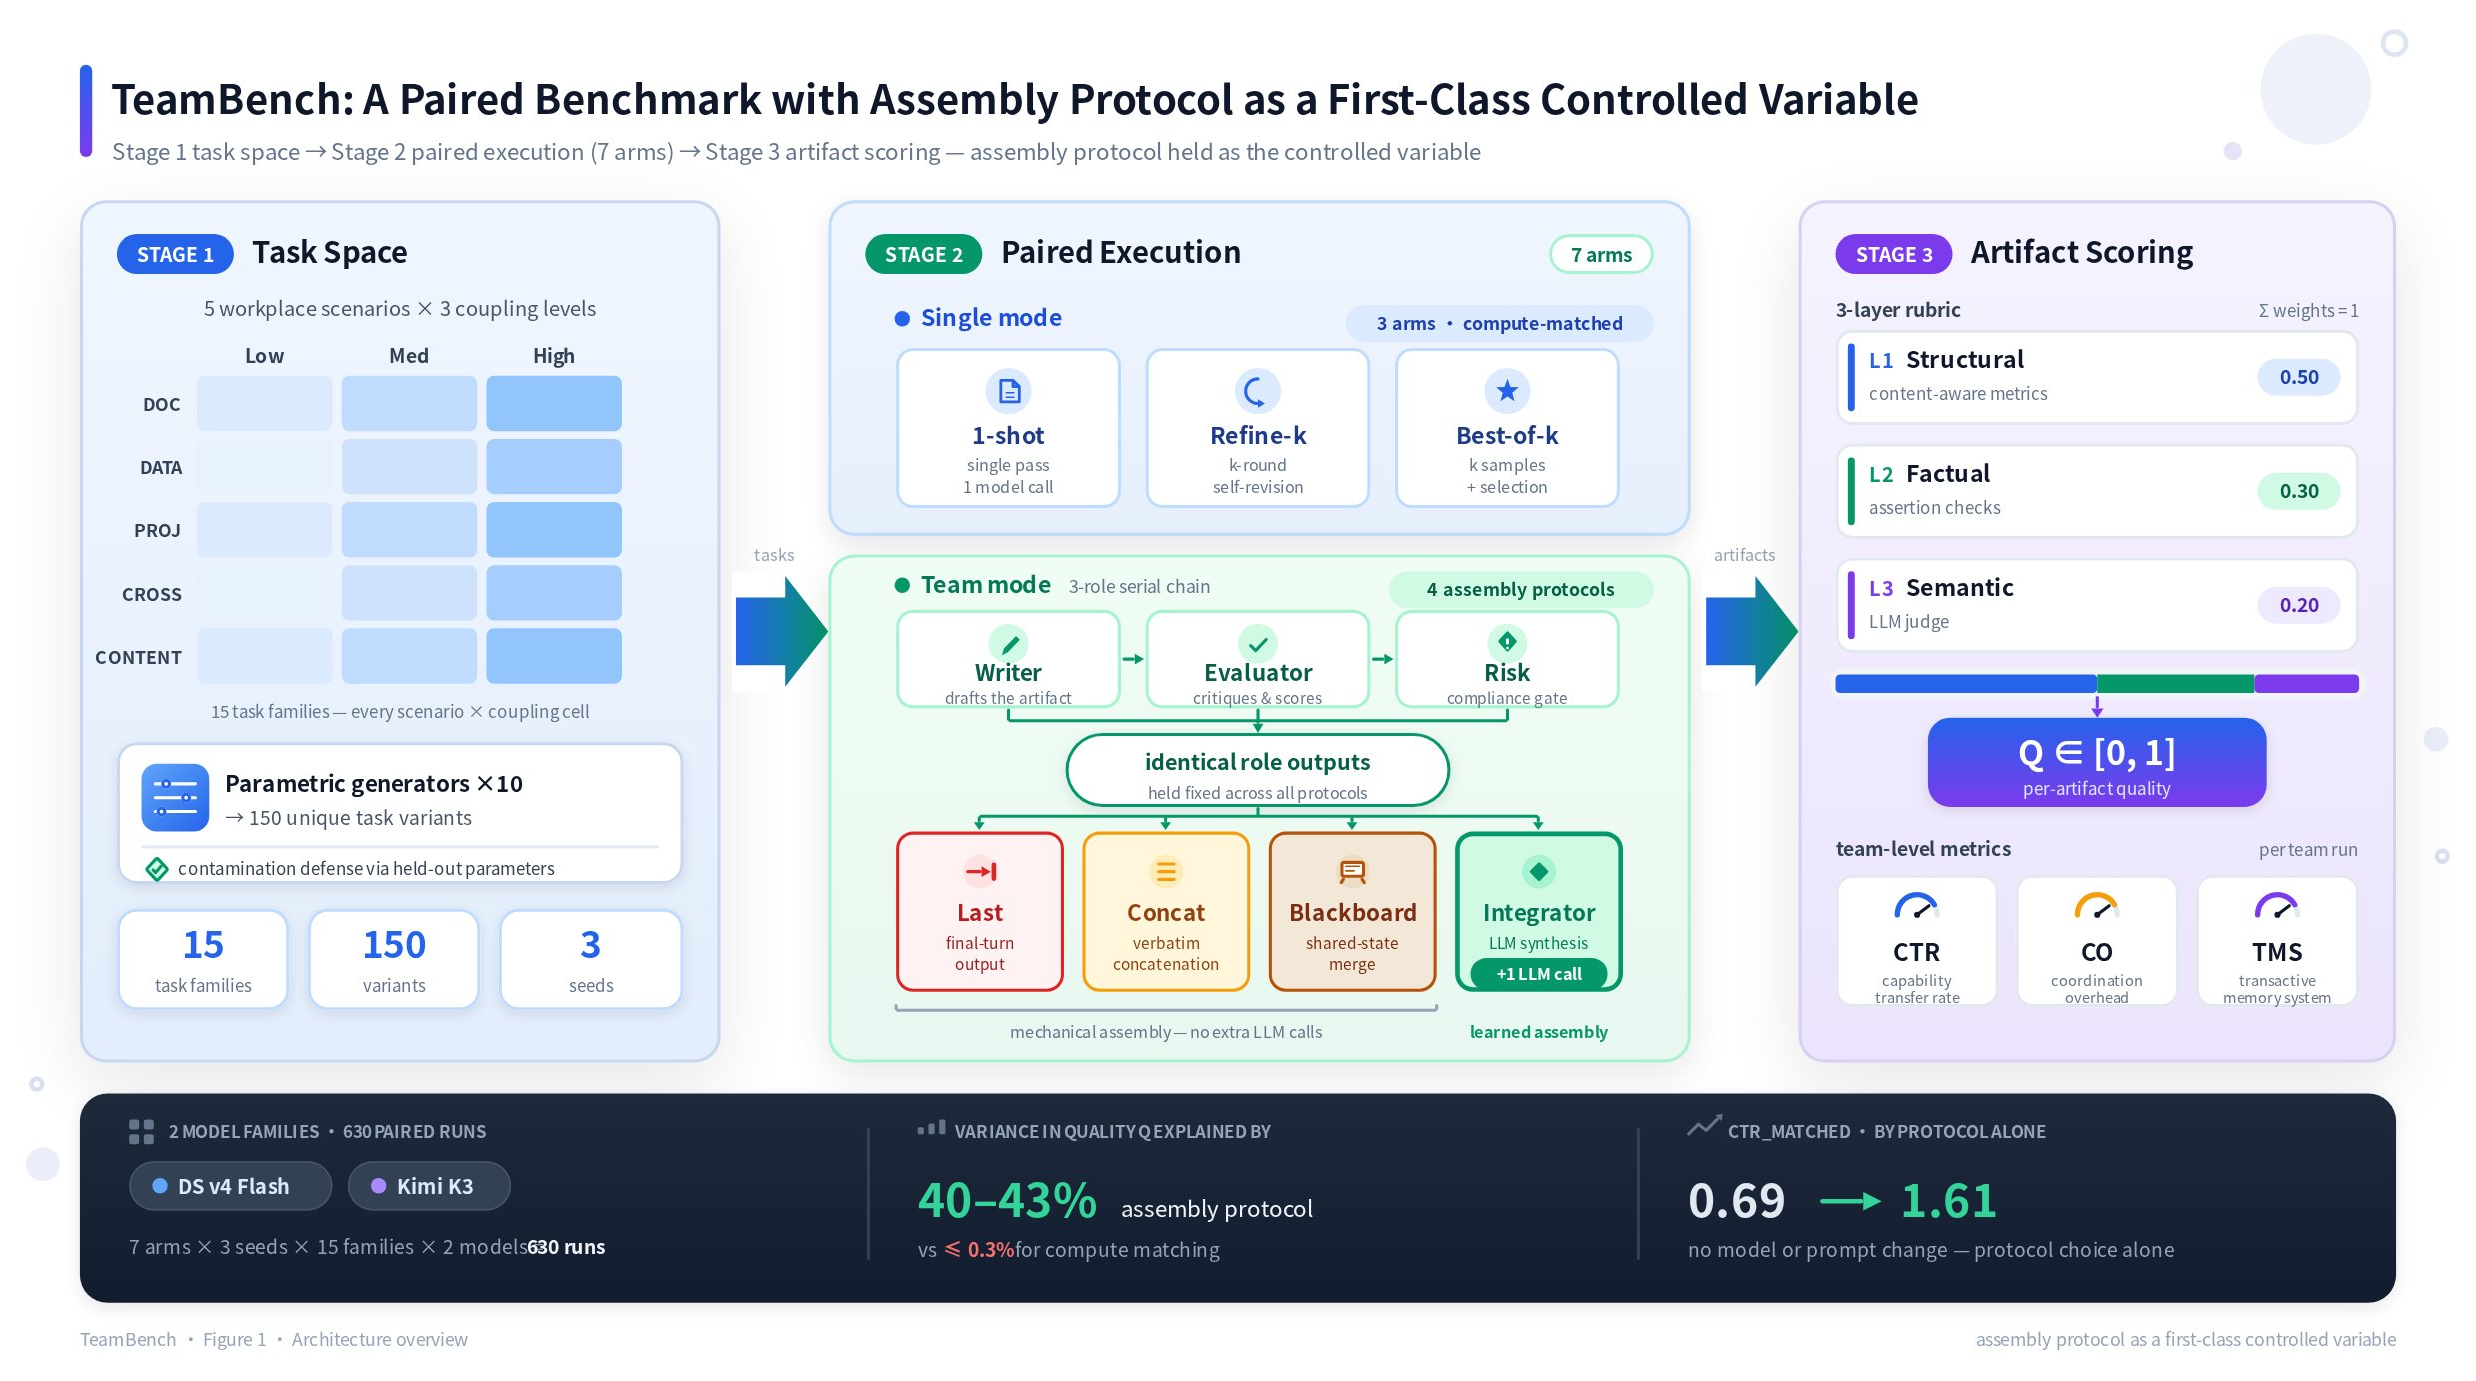
\includegraphics[width=\textwidth]{fig1_overview_wb.png}
\caption{\teambench{} overview. \textbf{Stage 1}---task space: 5 office scenarios $\times$ 3 coupling levels yield 15 task families, expanded to 150 variants by parameterized generators. \textbf{Stage 2}---paired execution over 7 arms: three single-mode baselines (1-shot, Refine-k, Best-of-k) and a team mode whose identical role outputs are assembled under 4 protocols (Last, Concat, Blackboard, Integrator). \textbf{Stage 3}---artifact scoring: three layers (L1 structural content-aware, L2 factual assertions, L3 semantic judge) produce team-level metrics CTR, CO, TMS.}
\label{fig:overview}
\end{figure*}

\begin{figure*}[t]
\centering
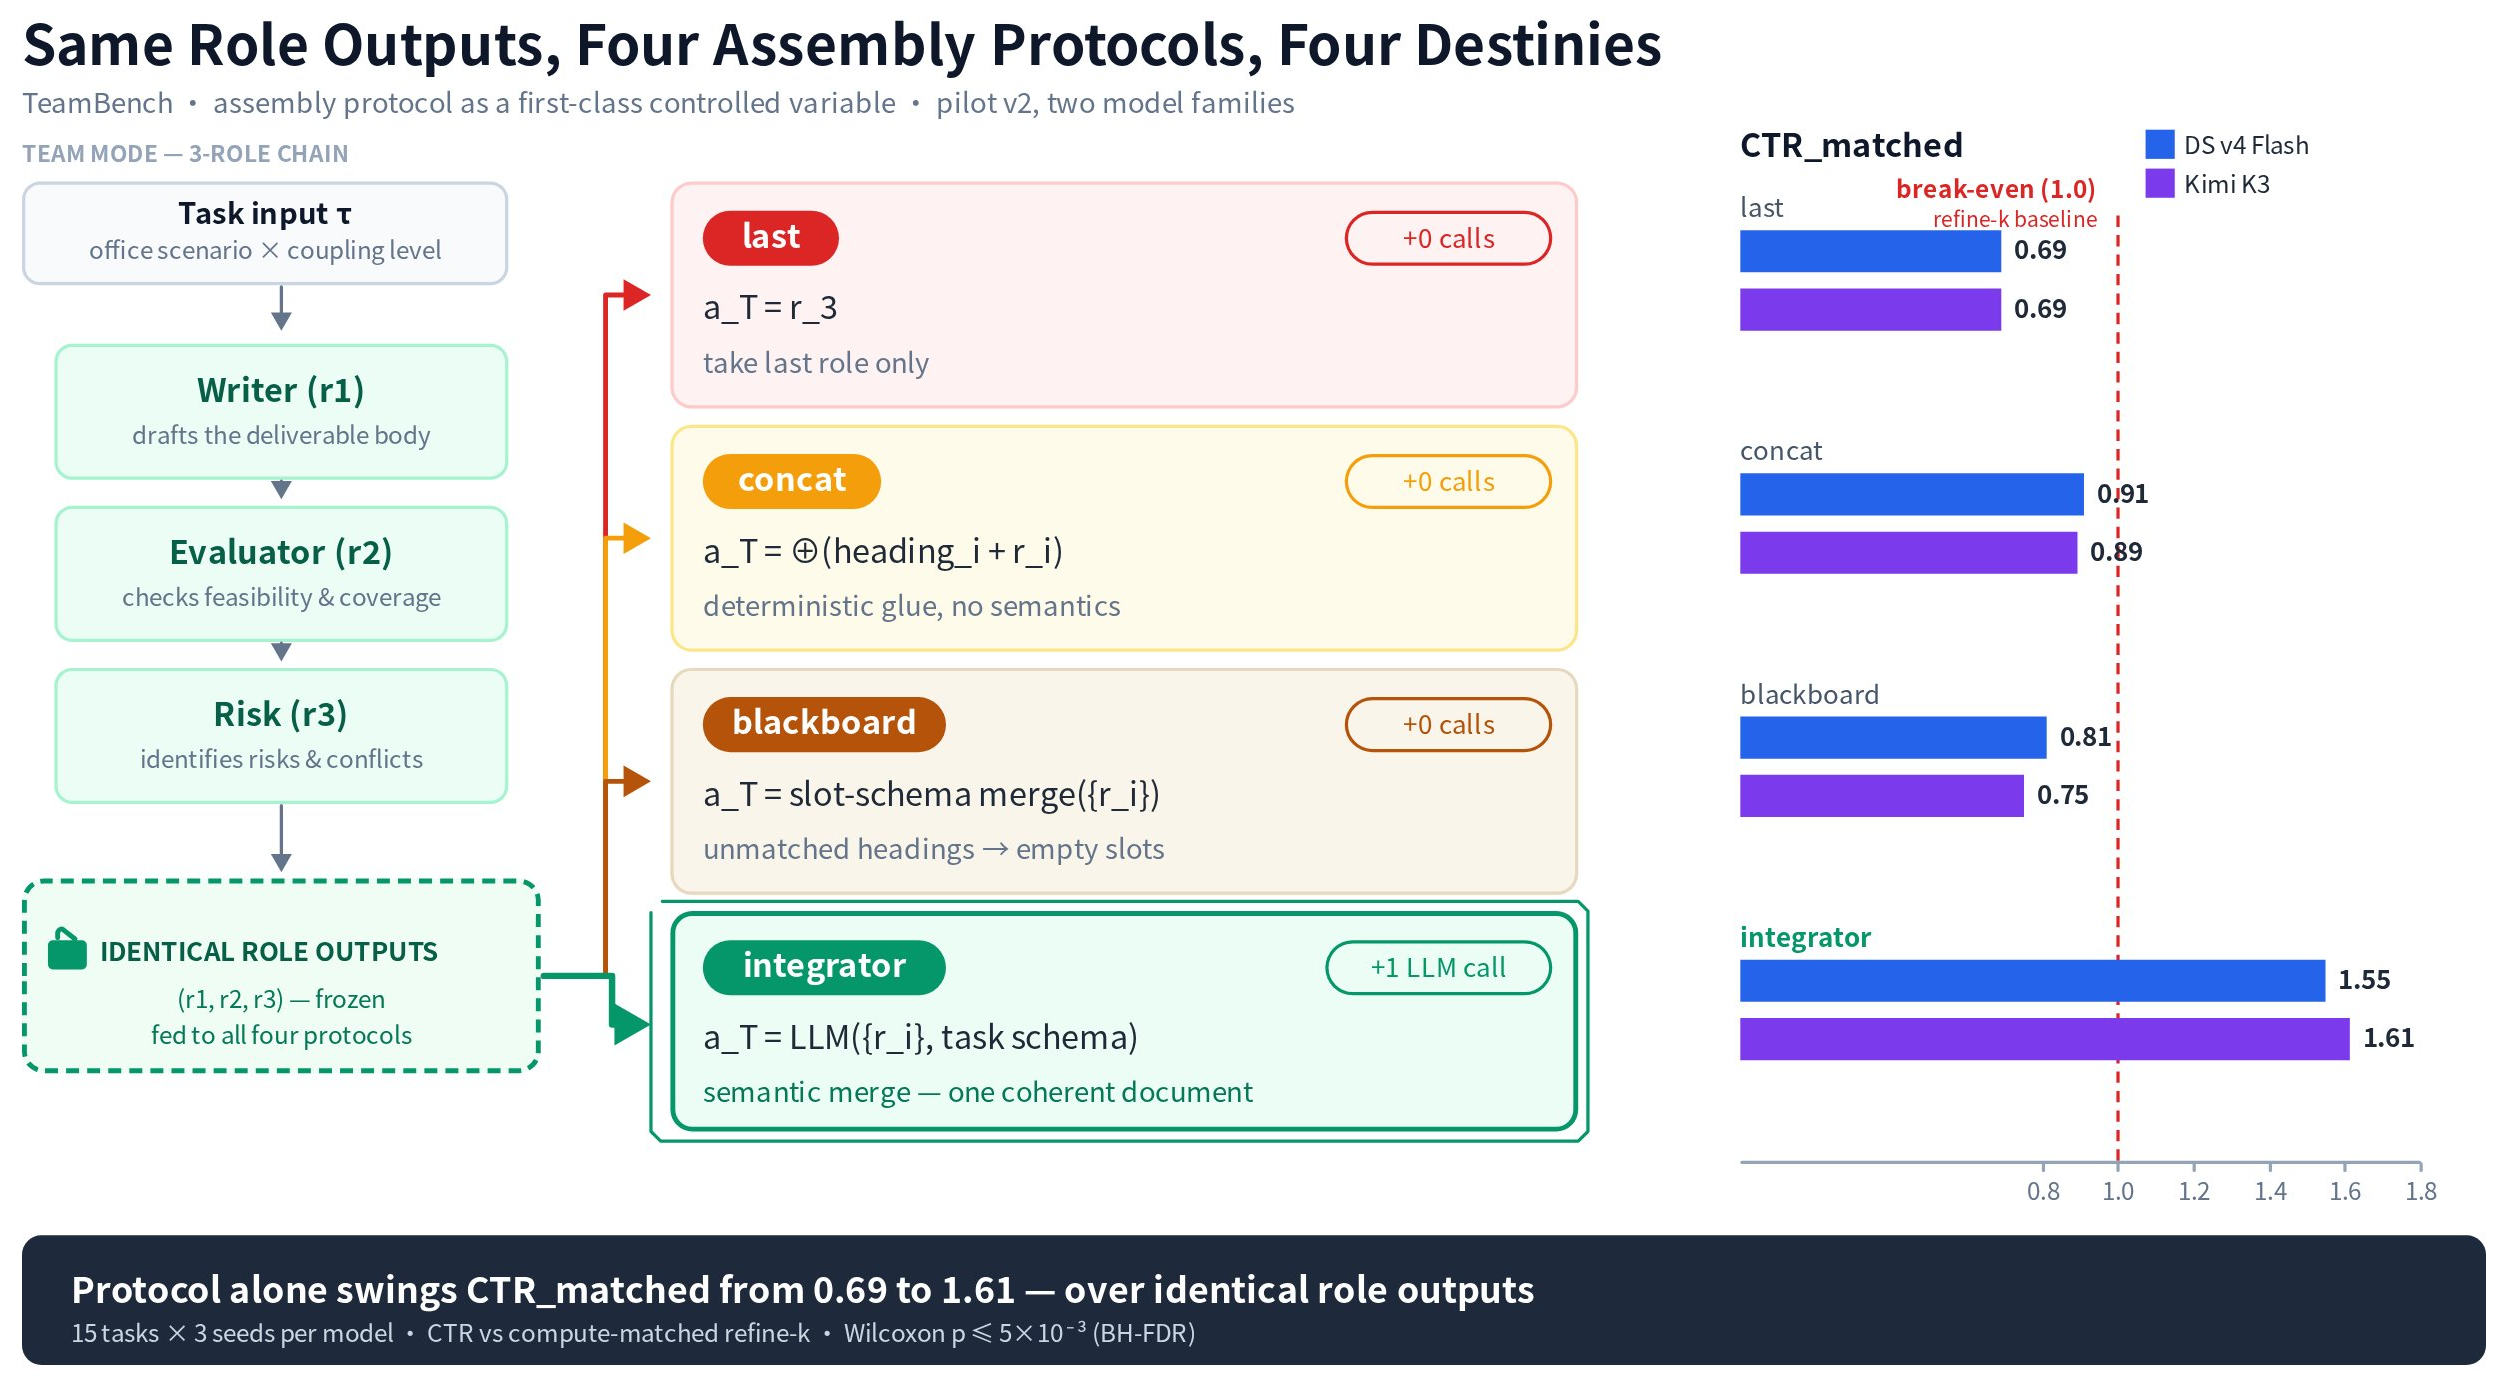
\includegraphics[width=\textwidth]{fig2_mechanism_wb.png}
\caption{The four assembly protocols over \emph{identical role outputs}. Only the integrator performs semantic merging of role content into the required artifact schema; the three mechanical protocols (last, concat, blackboard) rearrange or pass through role text without reconciling it against the schema. CTR\_matched by protocol alone spans 0.66--1.55 (geometric mean) across both model families, with no change to model, prompts, or role outputs.}
\label{fig:mechanism}
\end{figure*}

\subsection{Task space}
\label{sec:tasks}

5 workplace scenarios (DOCument writing, DATA aggregation, PROJect tracking, CROSS-functional coordination, CONTENT creation) $\times$ 3 coupling levels (LOW: parallel independent sub-tasks; MEDIUM: sequential dependencies; HIGH: parallel with cross-validation), yielding 15 task families. Each family is parameterized: inputs (e.g., team member records, table rows, conflict lists) are resampled and ground truths (L2 expected values, counts, sets) are deterministically recomputed. We verified per-family uniqueness of 10 variants and correctness of recomputed ground truths.

\subsection{Controlled variables}
\label{sec:variables}

\paragraph{Assembly protocol.} Four protocols applied to the \emph{same sequence of role outputs} $(r_1, \dots, r_k)$:

\begin{table}[h]
\centering
\small
\caption{Four assembly protocols over identical role outputs.}
\label{tab:protocols}
\setlength{\tabcolsep}{3pt}
\begin{tabular}{llc}
\toprule
Protocol & Definition & Added calls \\
\midrule
\code{last} & $a_T = r_k$ & 0 \\
\code{concat} & $a_T = \bigoplus_i \text{head}_i{+}r_i$ & 0 \\
\code{blackboard} & slot-schema merge & 0 \\
\code{integrator} & $a_T = \mathrm{LLM}(\{r_i\})$ & \textbf{+1} \\
\bottomrule
\end{tabular}
\end{table}

\code{last} is the engineering default of most frameworks; \code{concat} is deterministic concatenation; \code{blackboard} fills a structured slot schema (empty slots render placeholders); \code{integrator} performs a semantic merge via one dedicated LLM call whose cost is included in CO.

\paragraph{Compute-matched single baselines.}
\code{single\_refine\_k}: k sequential self-revisions (total LLM calls $= k$, matching the team). \code{single\_bon\_k}: k independent samples plus one selection call ($k{+}1$ calls; we attribute the marginal cost to the team-favorable side).

\subsection{Scoring protocol and the v2.2 measurement-integrity correction}
\label{sec:scoring}

\textbf{Correction 1 (L1 content-aware v2.1 $\to$ v2.2).} The v0 scorer checked only that required section headings existed. Under the \code{blackboard} protocol this made L1 trivially satisfiable: blackboard \emph{mechanically writes every required section heading}. Over 45 pilot runs under blackboard we observed 41 runs with empty sections, yet all received perfect L1 $= 1.0$ and therefore perfect $Q$, because 15/15 tasks lacked active L2 assertions (Correction 2). Scoring v2.2 adds a \emph{content-presence} gate: a section is counted only if the heading matches \emph{and} the body (excluding placeholders) has $\ge$8 normalized characters. Seven boundary cases are verified with unit tests.

\textbf{Correction 2 (L2 assertion migration v0.1 $\to$ v2).} The original 15 tasks declared ground-truth fields under ad-hoc keys that the v2 L2 rubric did not recognize; consequently L2 fell into the ``no assertions'' branch and returned 1.0 for every run. We migrated all 15 tasks and 150 parameterized variants to the shared \code{expected\_sets}/\code{expected\_values}/\code{expected\_counts} + \code{answer\_block\_schema} schema, verified 15/15 tasks have at least one L2 assertion, and ran acceptance checks: for every task the correct answer achieves L2 $\ge 0.99$, a deliberately incorrect answer scores strictly lower, and a missing answer block scores $\le 0.01$.

\subsection{Runner, breakpoint-resume, and balance guard}
\label{sec:runner}

The runner supports any combination of assembly protocol, single-baseline kind, and scoring-variant flags. Two reliability features: \textbf{breakpoint-resume} (per-(task,mode,seed) JSON files; restarts skip completed runs; summaries rebuilt deterministically) and a \textbf{balance guard} (queries provider balance every 5 runs, exits cleanly below a threshold), because pilot campaigns run overnight.

\section{Experiments}
\label{sec:experiments}

\paragraph{Data note.} All numbers below are pilot v2 final, \textbf{two model families}: DS v4 Flash and Kimi K3, each 15 tasks (migrated L2 assertions) $\times$ 3 seeds $\times$ 7 arms $=$ 315 runs (630 total), scoring v2.2, L3 judge off in the main tables. An earlier v1 pilot (same matrix, L2 inactive, Flash only) is used only for the scorer ablation in \S\ref{sec:scorer-validity}.

\subsection{Main result: assembly protocol flips the team effect}
\label{sec:main}

\begin{table*}[t]
\centering
\caption{Seven arms, pooled over 15 tasks $\times$ 3 seeds ($n{=}45$ per arm per model). No L3 judge. $\ctrm$ is the geometric mean over paired runs against each model's own refine-k arm (ratios with zero team scores are excluded from the geometric mean and reported as superscript zero-counts, e.g.\ $0.69^{(2)}$ = 2 zero-score runs of 45).}
\label{tab:main}
\small
\setlength{\tabcolsep}{4pt}
\begin{tabular}{lccccc|ccccc}
\toprule
& \multicolumn{5}{c|}{DS v4 Flash} & \multicolumn{5}{c}{Kimi K3} \\
Arm & $Q$ & L1 & L2 & TR & $\ctrm$ & $Q$ & L1 & L2 & TR & $\ctrm$ \\
\midrule
single (1-shot) & 0.606 & 0.515 & 0.759 & 1.00$\times$ & --- & 0.613 & 0.515 & 0.775 & 1.00$\times$ & --- \\
single\_refine\_k & 0.582 & 0.499 & 0.720 & 3.33$\times$ & (ref) & 0.637 & 0.543 & 0.795 & 4.27$\times$ & (ref) \\
single\_bon\_k & 0.584 & 0.506 & 0.715 & 4.27$\times$ & --- & 0.624 & 0.515 & 0.806 & 5.18$\times$ & --- \\
team\_last & 0.417 & 0.328 & 0.566 & 1.46$\times$ & \textbf{0.69}$^{(2)}$ & 0.420 & 0.324 & 0.580 & 2.53$\times$ & \textbf{0.66}$^{(3)}$ \\
team\_concat & 0.535 & 0.534 & 0.536 & 1.42$\times$ & 0.91$^{(1)}$ & 0.542 & 0.538 & 0.548 & 2.46$\times$ & 0.88$^{(2)}$ \\
team\_blackboard & 0.478 & 0.404 & 0.602 & 1.44$\times$ & 0.81$^{(2)}$ & 0.449 & 0.362 & 0.594 & 2.49$\times$ & 0.72$^{(3)}$ \\
team\_integrator & \textbf{0.881} & \textbf{0.964} & 0.741 & 2.14$\times$ & \textbf{1.55} & \textbf{0.905} & \textbf{0.978} & 0.785 & 4.44$\times$ & \textbf{1.50} \\
\bottomrule
\end{tabular}
\end{table*}

Geometric-mean $\ctrm$ with task-block bootstrap CIs for the integrator arm: Flash 1.55 $[1.32, 1.82]$, K3 1.50 $[1.26, 1.78]$; against the call-matched best-of-k baseline (both 4.2 LLM calls), the integrator reaches 1.56 (Flash) and 1.54 (K3), both $p<10^{-5}$ (Wilcoxon). All four team arms deviate from the refine-k baseline significantly on both models (two-sided Wilcoxon signed-rank with BH-FDR at $q=0.05$; Flash: last $p=1.0\times10^{-4}$, concat $p=5.1\times10^{-2}$, blackboard $p=4.6\times10^{-3}$, integrator $p=4.2\times10^{-7}$; K3: last $p=1.8\times10^{-5}$, concat $p=7.1\times10^{-3}$, blackboard $p=9.4\times10^{-5}$, integrator $p=1.2\times10^{-6}$).

\paragraph{Finding 1 (assembly flips the measured team effect).} On Flash, geometric-mean $\ctrm$ across 4 team protocols spans $\mathbf{0.69 \to 1.55}$ ($\Delta 0.86$) over \emph{identical role outputs}; on K3 the span is $\mathbf{0.66 \to 1.50}$ ($\Delta 0.84$). The integrator arm beats both compute-matched baselines on both models (vs.\ refine-k: Flash $p=4.2\times10^{-7}$, $d=+0.74$; K3 $p=1.2\times10^{-6}$, $d=+0.65$; vs.\ call-matched bon-k: 1.56 / 1.54, both $p<10^{-5}$); every mechanical protocol is significantly \emph{worse} than even the 1-shot single on both (K3 Cliff's $d$: last $-0.52$, blackboard $-0.42$, concat $-0.21$). The default engineering choice of last-role $=$ team output does not merely underperform---it produces a ``team-inferiority'' artifact ($\ctrm$ 0.69 / 0.66) that flips sign under integrator assembly.

\paragraph{Finding 2 (assembly dwarfs compute as a design axis).} Over the same set of role outputs, team-arm mean quality spans a range of \textbf{0.46} on Flash ($Q$ 0.417--0.881) and \textbf{0.49} on K3 (0.420--0.905), whereas single-arm compute strategies span only \textbf{0.025} on both (Flash 0.582--0.606; K3 0.613--0.637)---a $\sim$19$\times$ difference in range. Formally, in a pooled one-way ANOVA over all seven arms, arm identity explains $\eta^2 = 0.28$ (Flash) / $0.29$ (K3) of quality variance; the four team arms differ strongly from one another ($F=39.1$, $p=2.0\times10^{-19}$ Flash; $F=43.9$, $p=3.0\times10^{-21}$ K3) while the three single arms are statistically indistinguishable ($F=0.18$, $p=0.84$; $F=0.12$, $p=0.89$). We stress that these subset tests are descriptive---the two factors are not crossed in a single design, so we do not report a ratio of variance-explained figures. See Figure~\ref{fig:heatmap}(c).

\paragraph{Finding 2b (where the effect lives: layers).} The layer-wise decomposition in Table~\ref{tab:main} localizes the integrator's gain. Its L1 saturation rate is \textbf{95.6\%} (Flash) / \textbf{97.8\%} (K3), versus 26.7--31.1\% for the single arms; layer-wise $\ctrm$(L1) reaches 1.97 / 2.04. On the factual layer, however, the integrator is at \emph{parity} with single agents ($\ctrm$(L2) vs.\ 1-shot: 1.05, $p=0.87$ Flash; 1.04, $p=0.89$ K3), while every mechanical protocol significantly \emph{degrades} it ($\ctrm$(L2) 0.69--0.78, all $p<0.05$). TMS (perfect structure \emph{and} facts) passes for 46.7\% / 55.6\% of integrator runs versus $\le$22.2\% for any single arm and 6.7\% for all mechanical arms. The correct reading is not that teams generate better \emph{facts} than individuals, but that assembly governs whether the facts already produced by the roles survive into the artifact: mechanical assembly loses them; semantic integration preserves them and restores the schema-compliant structure that singles rarely produce.

\paragraph{Finding 3 (team gains survive compute-matching).} On Flash, the integrator burns 2.14$\times$ tokens vs.\ the 1-shot single and reaches $\ctrn$ 1.52, while refine-k (3.33$\times$) and bon-k (4.27$\times$) burn \emph{more} compute yet score \emph{below} the 1-shot single ($\ctrn$ 0.96). K3 sharpens this result: its stronger self-revision lifts refine-k to $\ctrn$ 1.08, yet the integrator still reaches $\ctrn$ 1.72. The integrator's advantage also holds under the strictest call-matched comparison (vs.\ bon-k, both 4.2 LLM calls): $\ctrm$ 1.56 (Flash) / 1.54 (K3), both $p<10^{-5}$. More sampling or more revision rounds does not substitute for semantic integration on either model.

\paragraph{Finding 4 (mechanical assembly fails at semantics; L2 localizes where).} On both Flash and K3, concat's factual layer (L2 0.536 / 0.548) falls \emph{below} last's (0.566 / 0.580): the answer-block extractor takes the last \code{json} block, which in a naive concatenation is the final role's \emph{partial} block, while earlier roles' numeric content is stranded. The integrator is the only protocol that reliably aggregates all roles' numbers into one consistent answer block.

\paragraph{Finding 5 (cross-model replication, with honest failure cases).} The effect structure replicates across two model families: the arm ordering (integrator $\gg$ concat $>$ blackboard $>$ last) is identical; all four team arms deviate significantly from refine-k on both models under BH-FDR; and per-coupling integrator $\ctrm$ CIs exclude 1.0 in all six cells, though the high-coupling cells are marginal (lower CI bounds 1.05--1.06 with $n{=}15$ per cell). The integrator is not uniformly superior: it scores below the 1-shot single on 3/15 tasks on Flash and 4/15 on K3 (e.g.\ \code{t-CONTENT-H-03}, \code{t-CROSS-L-01}). A single-case study makes the mechanism vivid (K3, \code{t-DATA-L-01}, seed 0; Figure~\ref{fig:case})---we present it as an illustrative extreme, not a typical case: the same two role outputs score $Q=1.00$ under the integrator, 0.42 under concat, and \textbf{0.00 under both last and blackboard}---while every single-mode baseline lands at 0.38--0.79. The capability was present in the role outputs all along; the assembly protocol alone determined whether it survived to the artifact.

\begin{figure*}[t]
\centering
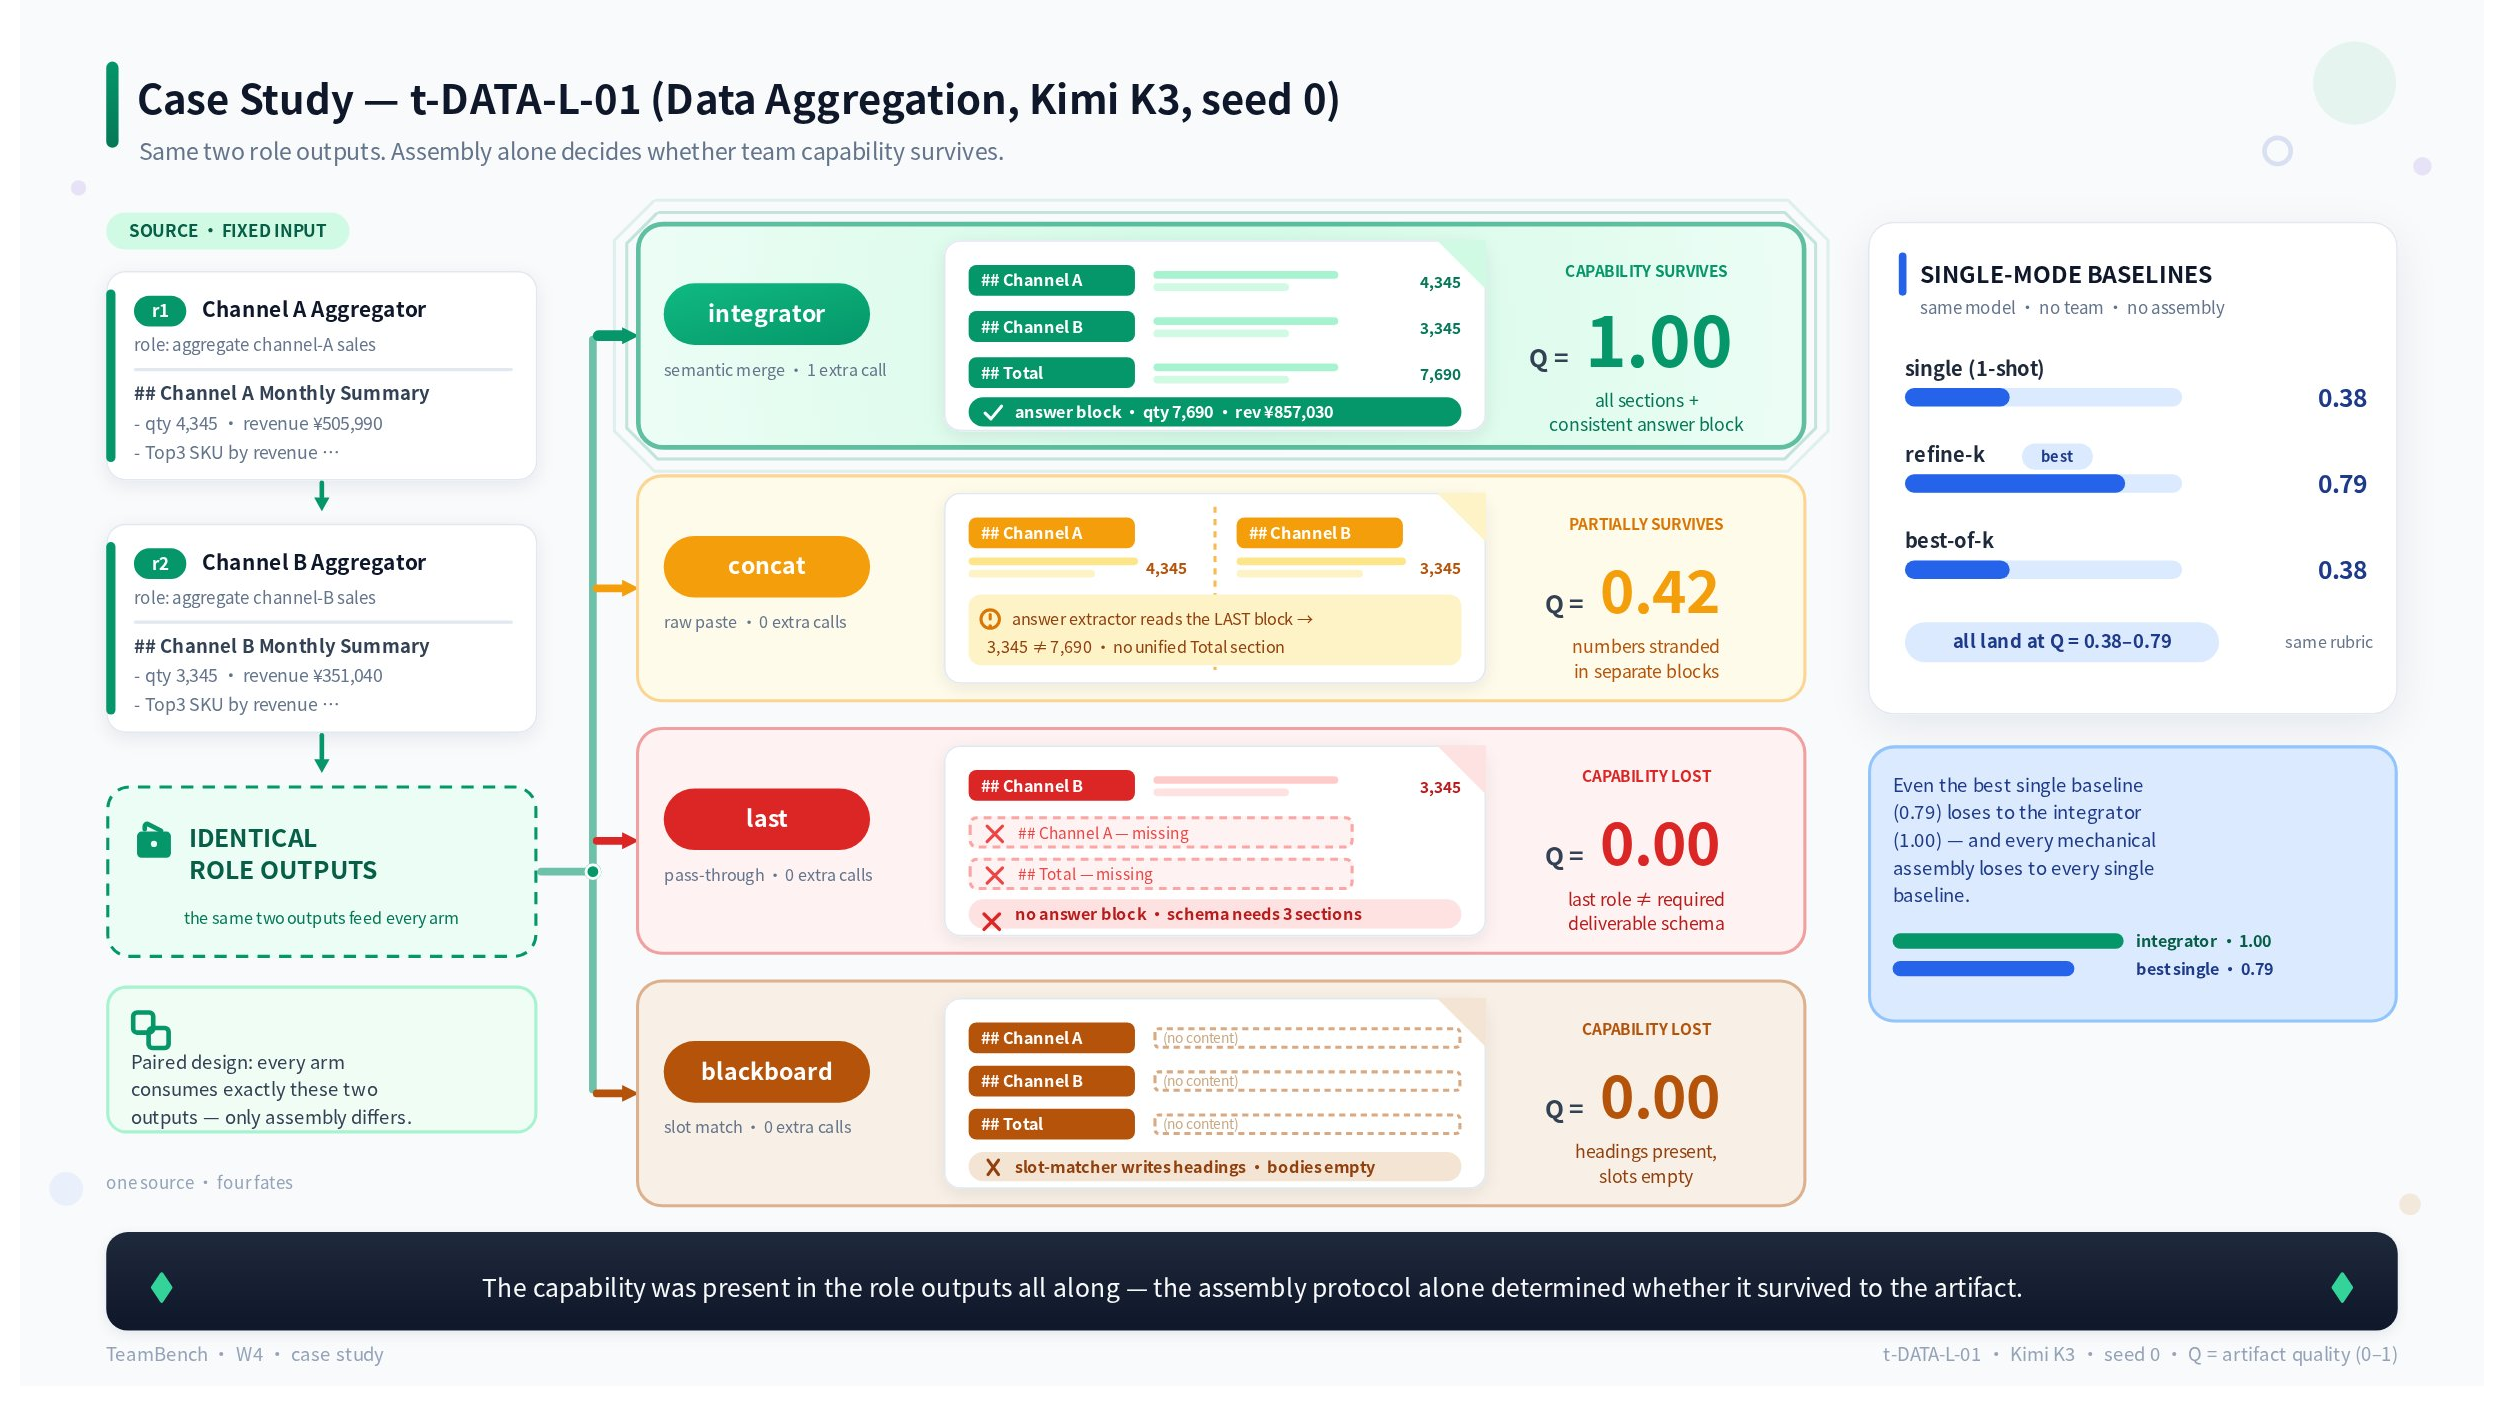
\includegraphics[width=\textwidth]{fig_case_study_wb.png}
\caption{Case study \code{t-DATA-L-01} (DATA aggregation, low coupling; Kimi K3, seed 0). The same two role outputs (channel-A and channel-B aggregators) feed all four assembly arms. The integrator merges both channels into the three-section schema with a consistent answer block ($Q{=}1.00$); concat strands each channel's numbers in separate blocks that the answer extractor cannot reconcile ($Q{=}0.42$); last passes through only the final role, missing two required sections ($Q{=}0.00$); blackboard writes the required headings but leaves slot bodies empty ($Q{=}0.00$). Every single-mode baseline lands at $Q = 0.38$--$0.79$ on the same task and rubric.}
\label{fig:case}
\end{figure*}

\subsection{CTR after controlling assembly, by coupling}
\label{sec:coupling}

\begin{table*}[t]
\centering
\caption{Quality by coupling level (5 tasks $\times$ 3 seeds per cell), both models.}
\label{tab:coupling}
\small
\setlength{\tabcolsep}{3.5pt}
\begin{tabular}{lcccccc|cccccc}
\toprule
& \multicolumn{6}{c|}{DS v4 Flash} & \multicolumn{6}{c}{Kimi K3} \\
Coupling & single & ref-k & last & concat & \textbf{integ.} & black. & single & ref-k & last & concat & \textbf{integ.} & black. \\
\midrule
Low & 0.603 & 0.522 & 0.404 & 0.537 & \textbf{0.905} & 0.500 & 0.604 & 0.657 & 0.444 & 0.625 & \textbf{0.919} & 0.482 \\
Medium & 0.595 & 0.608 & 0.339 & 0.493 & \textbf{0.876} & 0.447 & 0.579 & 0.586 & 0.321 & 0.432 & \textbf{0.872} & 0.292 \\
High & 0.621 & 0.615 & 0.510 & 0.574 & \textbf{0.861} & 0.488 & 0.656 & 0.669 & 0.494 & 0.569 & \textbf{0.925} & 0.573 \\
\midrule
$\ctrm$ (integ., geo.) & \multicolumn{6}{c|}{1.69 / 1.46 / 1.51} & \multicolumn{6}{c}{1.43 / 1.55 / 1.52} \\
\bottomrule
\end{tabular}
\end{table*}

The integrator advantage is \textbf{uniform across coupling levels on both models} (all six cells $p < 0.005$; all six geometric-mean bootstrap CIs exclude 1.0, though the high-coupling cells are marginal with lower bounds 1.05--1.06 at $n{=}15$ per cell); no Simpson paradox emerges when pooling. Notably, an earlier ``coupling law'' (CTR increasing monotonically with coupling) does \textbf{not} reappear once assembly is controlled: it was an artifact of last-role assembly interacting with role ordering, not a property of teams.

\begin{figure*}[t]
\centering
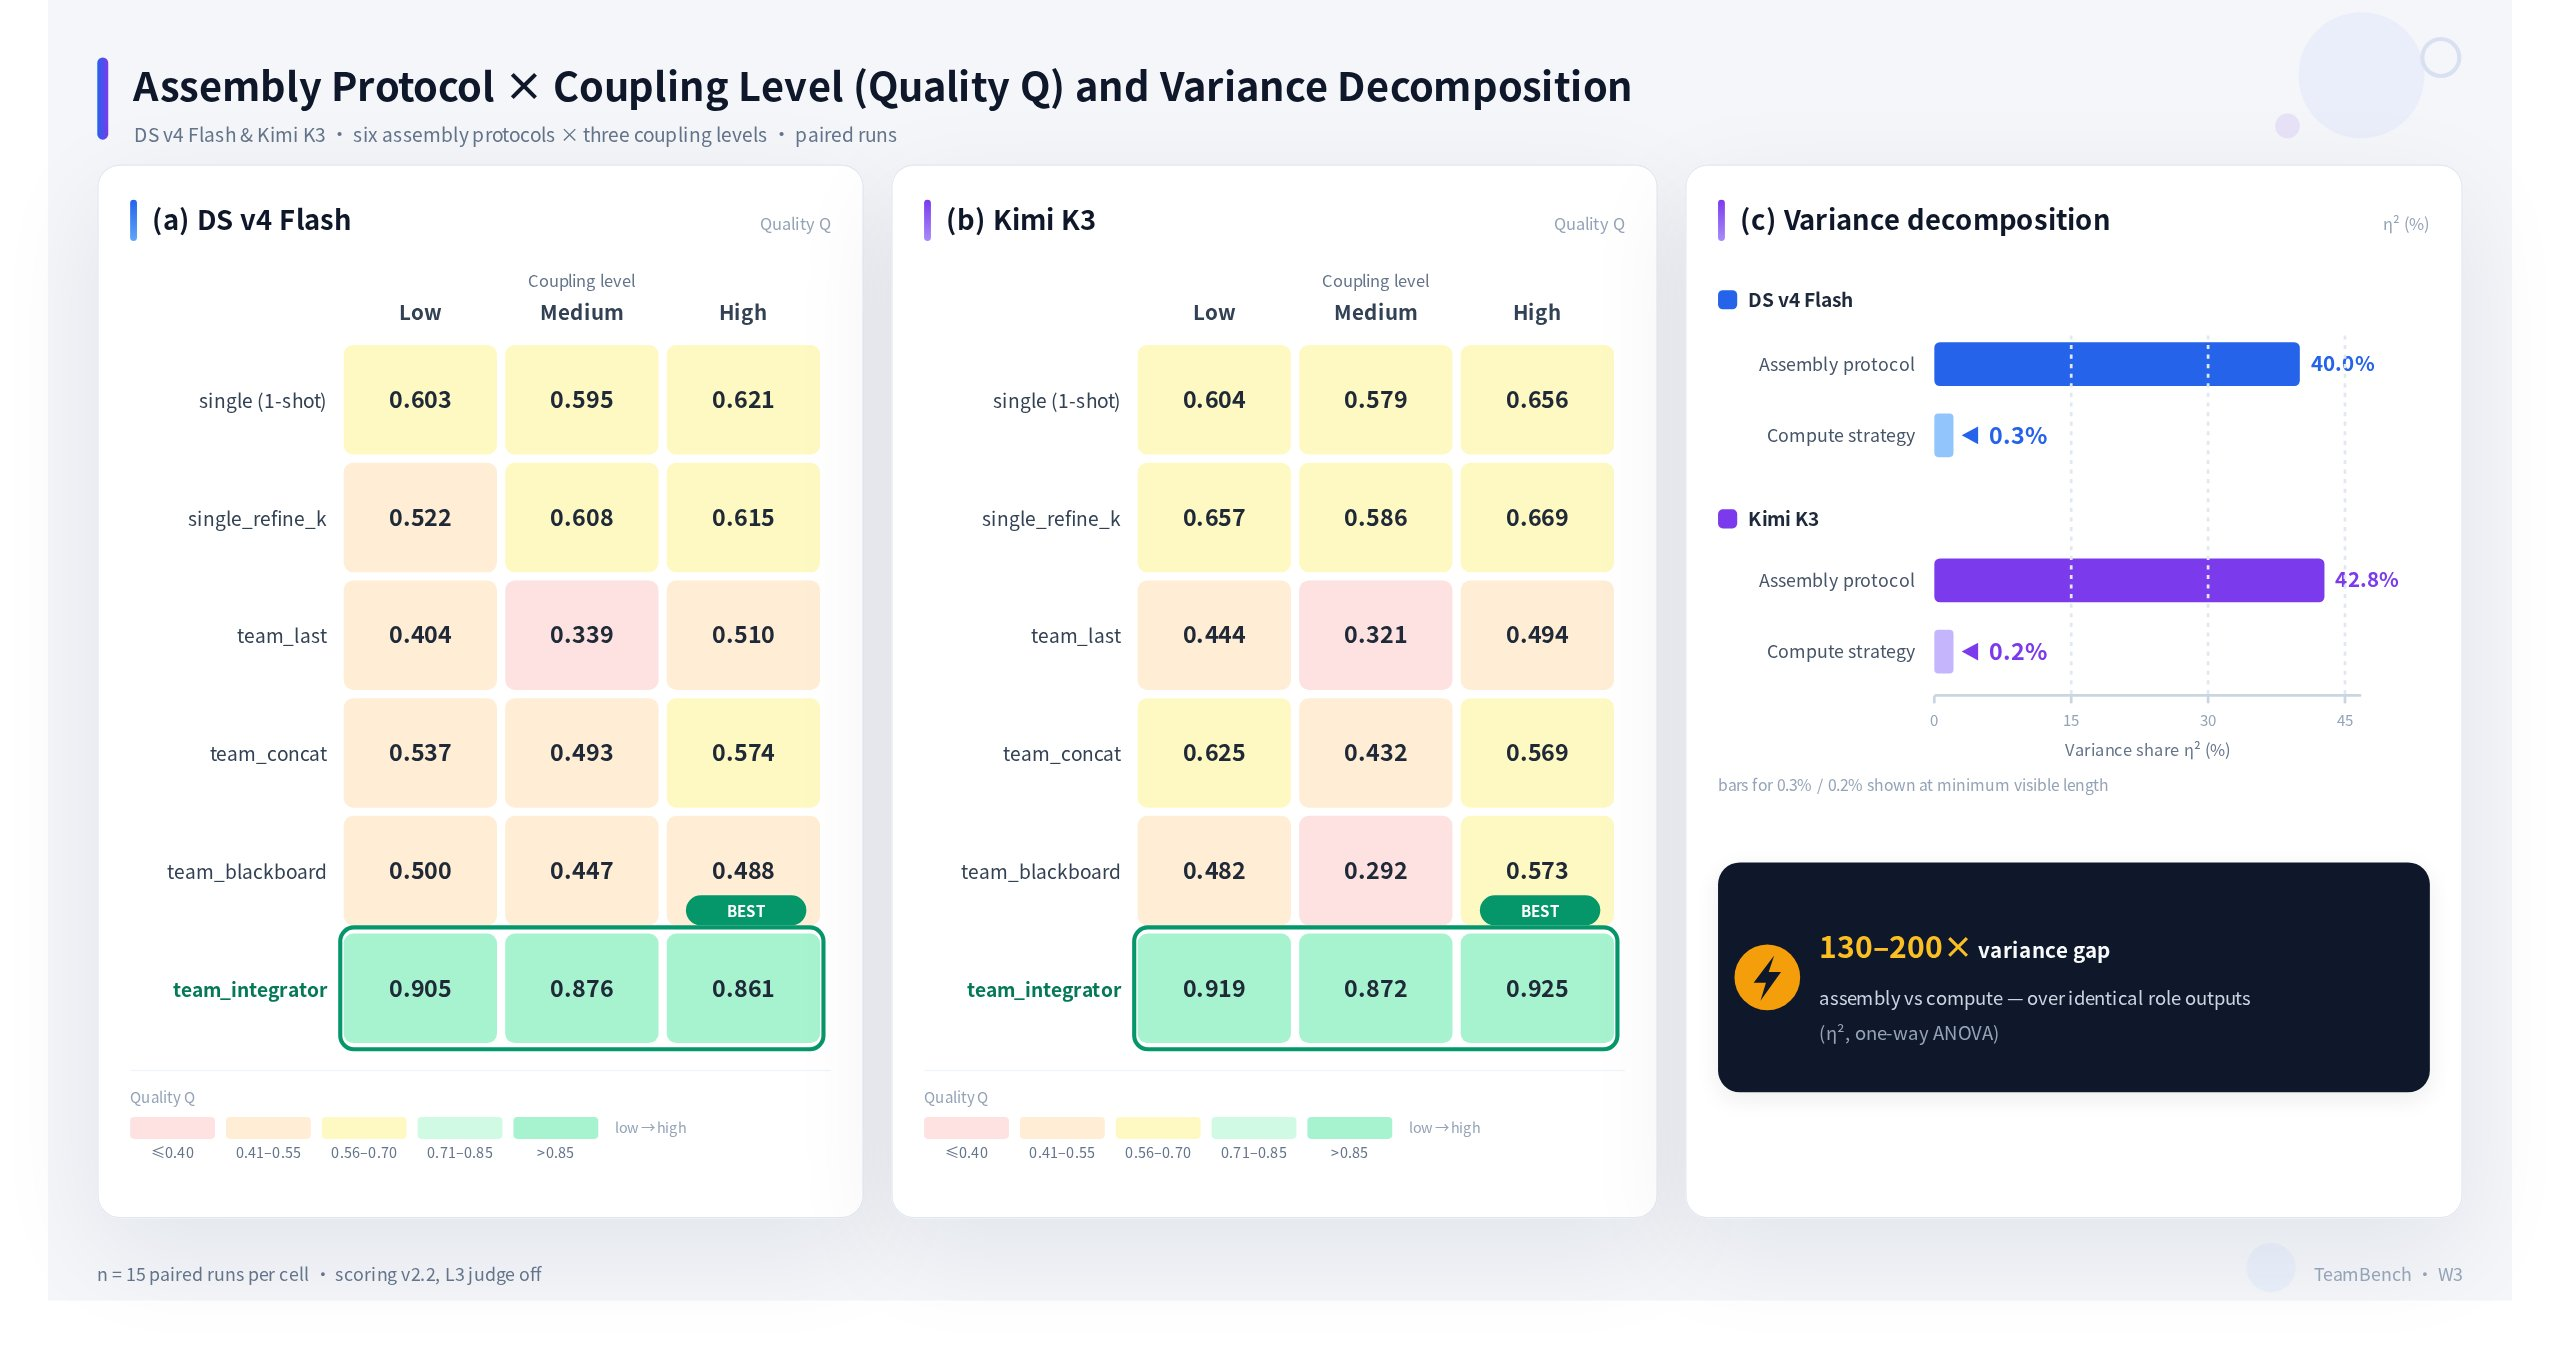
\includegraphics[width=\textwidth]{fig4_assembly_coupling_wb.png}
\caption{(a)(b) Quality $Q$ by assembly protocol $\times$ coupling level (15 paired runs per cell), DS v4 Flash and Kimi K3 side by side. The integrator row dominates every coupling level on both models while all mechanical protocols fall below both single baselines. (c) Range of arm means: assembly protocol spans 0.417--0.881 (Flash) and 0.420--0.905 (K3) over identical role outputs, whereas compute strategy spans only 0.582--0.606 and 0.613--0.637---a $\sim$19$\times$ difference in range, replicated across model families.}
\label{fig:heatmap}
\end{figure*}

\begin{figure}[t]
\centering
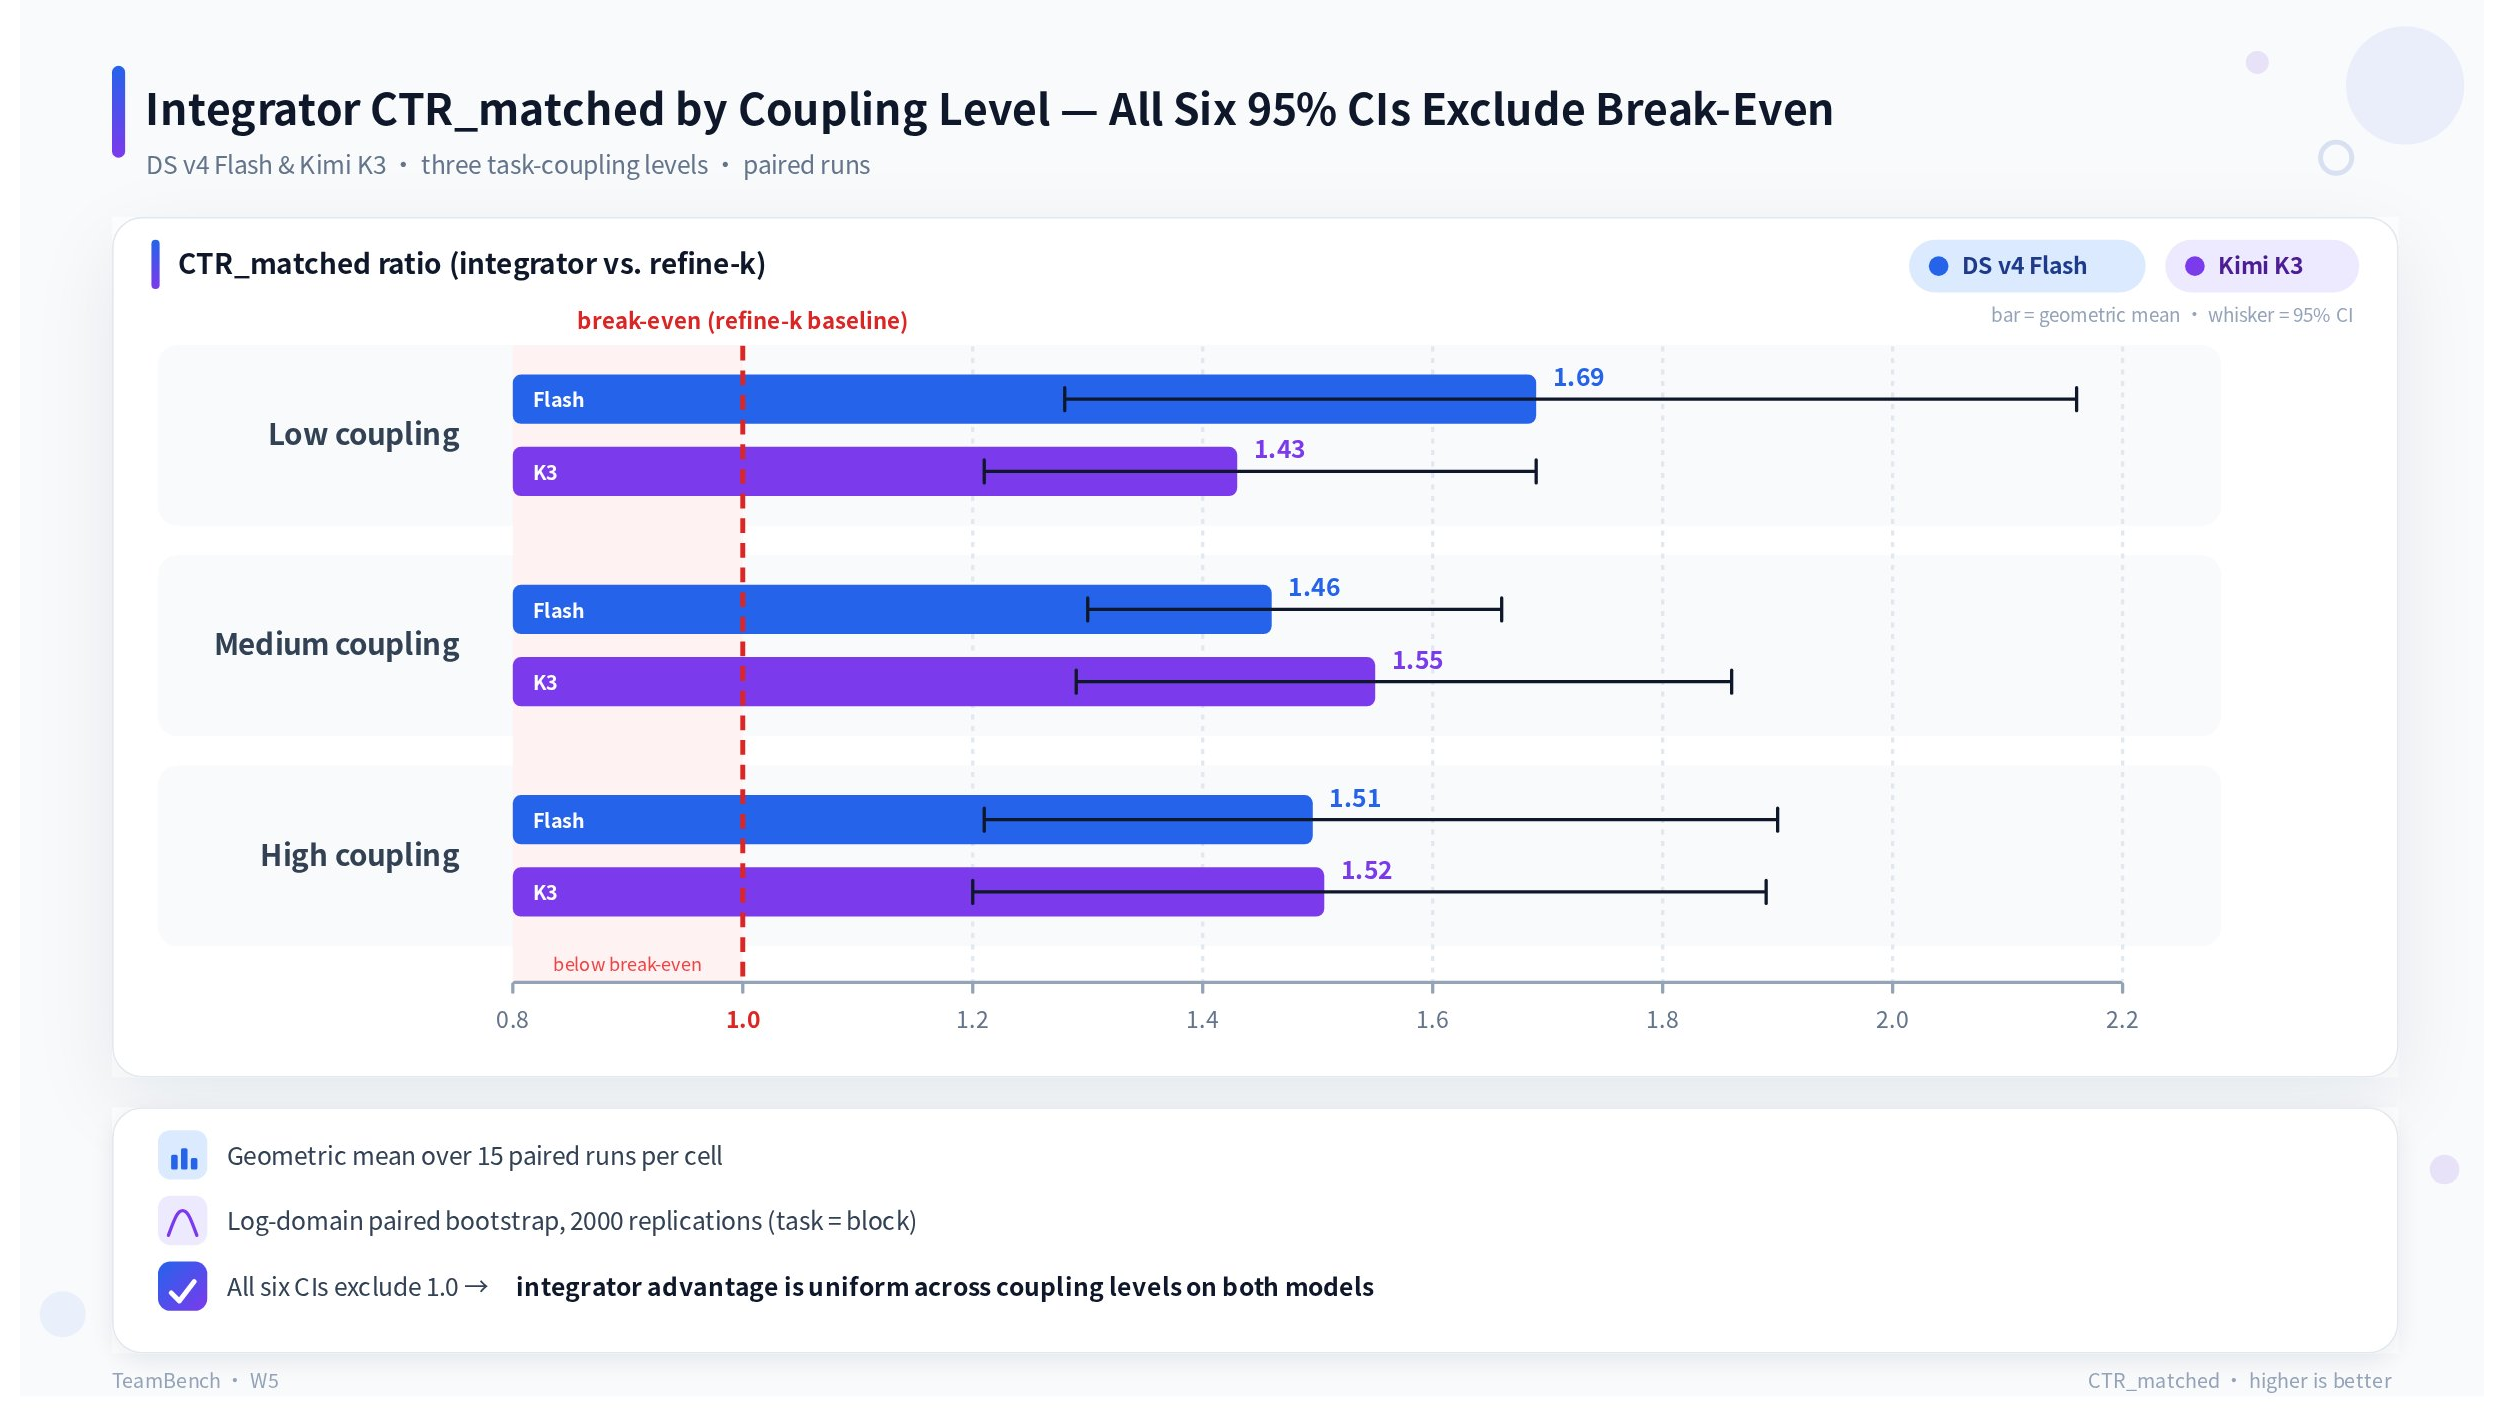
\includegraphics[width=\columnwidth]{fig5_ctr_matched_wb.png}
\caption{Integrator $\ctrm$ by coupling level, both models (geometric mean, log-domain paired bootstrap 95\% CI, $n=15$ per level per model). All six CIs exclude the break-even line at 1.0.}
\label{fig:ctr}
\end{figure}

\subsection{Scorer validity}
\label{sec:scorer-validity}

We document two scorer ablations in place of a full human study (left for the full experiment).

\paragraph{L1 v0 (title-only) vs.\ v2.2 (content-aware).} In the v1 pilot, blackboard mechanically rendered every required heading, 41/45 runs had empty sections, and all 45 received perfect L1 $=1.0$---flipping the arm from ``best'' to ``below average'' once the content gate landed. This incident is itself evidence that automated structural rubrics without content gates are gameable by construction.

\paragraph{L2 off (v1) vs.\ L2 on (v2), same task matrix.} Enabling L2 lowered every arm's absolute $Q$ (single $0.692 \to 0.606$; integrator $0.958 \to 0.881$) but \emph{increased} the integrator's relative advantage ($\ctrm$ $1.54 \to 1.55$; $d$ $+0.59 \to +0.74$): the numeric layer rewards exactly the cross-role aggregation that only the integrator performs. Findings F1--F4 are robust to the L2 switch.

\paragraph{L3 judge on/off ablation (cross-family judges).}
We re-scored the full seed-0 subsample of both models (15 tasks $\times$ 7 arms $\times$ 2 models $=$ 210 runs) with the L3 judge enabled, using a \emph{cross-family judge matrix} to avoid same-family bias: Flash artifacts judged by kimi-k3, K3 artifacts judged by deepseek-v4-pro; each run judged twice independently. Judge test-retest agreement is good and nearly identical across judges (Flash: 74\% exact match, Spearman $\rho = 0.855$; K3: 74\%, $\rho = 0.824$). \textbf{The arm ordering is perfectly stable under L3}: Spearman between L3-off and L3-on arm ranks is $1.000$ on both models---the integrator remains first, mechanical protocols remain last. Absolute $Q$ rises slightly for non-ceiling arms ($+0.02$--$0.05$; the judge is mildly lenient) while the integrator is unchanged ($\Delta \le 0.002$, ceiling effect); $\ctrm(\text{integrator})$ moves from 1.60 to 1.49 (Flash) and 1.38 to 1.29 (K3)---both far above 1. Findings F1--F5 are robust to the L3 switch: the assembly effect is not an artifact of deterministic-only scoring.

\subsection{Statistical details}
\label{sec:stats}

All comparative claims use the two-sided Wilcoxon signed-rank test on paired per-(task,seed) differences, with BH-FDR correction at $q=0.05$ where multiple arms are compared. CTR is reported as the geometric mean over paired runs (ratio scale); paired runs with zero team scores are excluded from the geometric mean and their counts reported explicitly. CTR CIs use 5000 task-block bootstrap replications (task $=$ block). Effect sizes are Cliff's $d$ on paired quality differences.

\section{Discussion}
\label{sec:discussion}

\paragraph{For practitioners.} The data support three decision rules (``when to use a team and which assembly''):

\begin{table}[h]
\centering
\small
\caption{Practitioner decision table.}
\setlength{\tabcolsep}{3pt}
\begin{tabular}{llp{3.4cm}}
\toprule
Scenario & Recommendation & Why \\
\midrule
Any team use & Never ship last-role & Last-role loses 31--34\% of compute-matched quality on both models. \\
Team justified & Integrator assembly & $\ctrm \approx 1.5\times$ at every coupling level (Low 1.69/1.43, Med 1.46/1.55, High 1.51/1.52); $\sim$2$\times$ token cost. \\
No team & Single + 1-shot & Refine-k / bon-k do not beat 1-shot on Flash; on K3 refine-k gains 8\% for 4.3$\times$ tokens. \\
\bottomrule
\end{tabular}
\end{table}

\paragraph{For framework developers.} Expose assembly protocol as a first-class knob. In their default configurations, common group-chat and sequential-pipeline patterns (AutoGen group chat, CrewAI sequential, LangGraph edge endpoints) typically return the last agent's reply as the final answer unless the developer wires in explicit aggregation---an informal survey of the three frameworks' defaults, not a controlled trace study. A built-in \code{team.finalize()} with token-cost attribution would align research and production practices.

\paragraph{For benchmark designers.} Three lessons: (1) Report assembly protocol the same way you report temperature---it can swing the measured effect more than the model does. (2) Structural rubrics require a content gate; mechanical headings are always a gaming risk when evaluation is automated. (3) Compute-matched baselines are not optional for ``multi vs.\ single'' papers.

\section{Limitations}
\label{sec:limitations}

\begin{enumerate}
\item \textbf{Monolingual, Chinese-heavy.} Task descriptions and role prompts are in Chinese; artifact rubrics check Chinese-section headings. An English subset is deferred to follow-up work.
\item \textbf{Synthetic office tasks.} Seeded from real documents but synthetic; no ground-truth downstream outcomes.
\item \textbf{Fixed team topology.} Serial handoff with fixed role templates; no self-organizing role discovery, no parallel tool usage, no agent churn.
\item \textbf{Model coverage.} Two model families completed (DS v4 Flash, Kimi K3, 630 runs); the assembly effect, arm ordering, and variance structure replicate across both. Conclusions about ``model capability'' are necessarily limited to these two families.
\item \textbf{Integrator prompt visibility.} The integrator's system prompt receives the task's required-section schema, as any final-stage editor in a real pipeline would; its near-perfect L1 saturation is therefore partly attributable to rubric visibility. The layer-wise decomposition (\S\ref{sec:main}, Finding 2b) partially controls for this---the factual layer (L2), whose schema is \emph{not} disclosed in a gameable way, shows parity rather than gain---but a fully rubric-blind integrator ablation remains future work, and the structural share of the integrator's advantage should be read with this caveat.
\item \textbf{L3 judge.} Main tables score with L3 off (renormalized L1/L2); \S\ref{sec:scorer-validity} reports a completed L3-on ablation over the full seed-0 subsample (210 runs, cross-family judges, two rounds each) showing the arm ordering is perfectly stable (Spearman $= 1.000$ on both models).
\item \textbf{Open-loop runtime.} No mid-run budget halts, no human-in-the-loop interventions.
\end{enumerate}

\section{Conclusion}
\label{sec:conclusion}

The field has been asking ``do LLM teams outperform individuals,'' but our controlled experiment shows that on identical role outputs, most of the variance in the answer comes from \emph{how the team's output is assembled}, not from additional compute or the task's coupling. Across four assembly protocols and two model families (630 runs), the measured team effect flips sign with the protocol alone: geometric-mean $\ctrm$ spans 0.69--1.55 (Flash) and 0.66--1.50 (K3), and the integrator arm beats both compute-matched baselines on both (vs.\ best-of-k at identical call counts: 1.56 / 1.54), while naive last-role assembly---a common engineering default---manufactures ``team inferiority.'' Layer-wise decomposition sharpens the message: mechanical assembly destroys the factual content that roles produced; semantic integration preserves it and restores schema-compliant structure. Multi-agent papers that do not report their assembly protocol are reporting a pipeline artifact as a property of teams.

\balance

\bibliographystyle{ACM-Reference-Format}
\bibliography{refs}

\end{document}
